\subsection{Mockups}
Users can interact with our system through the mobile application, the website and the display located inside the car.

\subsubsection*{View available car information in mobile application} This mockup shows how the information of an available car (charge level and distance from the client) can be displayed in the mobile app. The logged client has the possibility to reserve the car by tapping on the "Reserve" button.
\begin{figure}[hp]
\centering
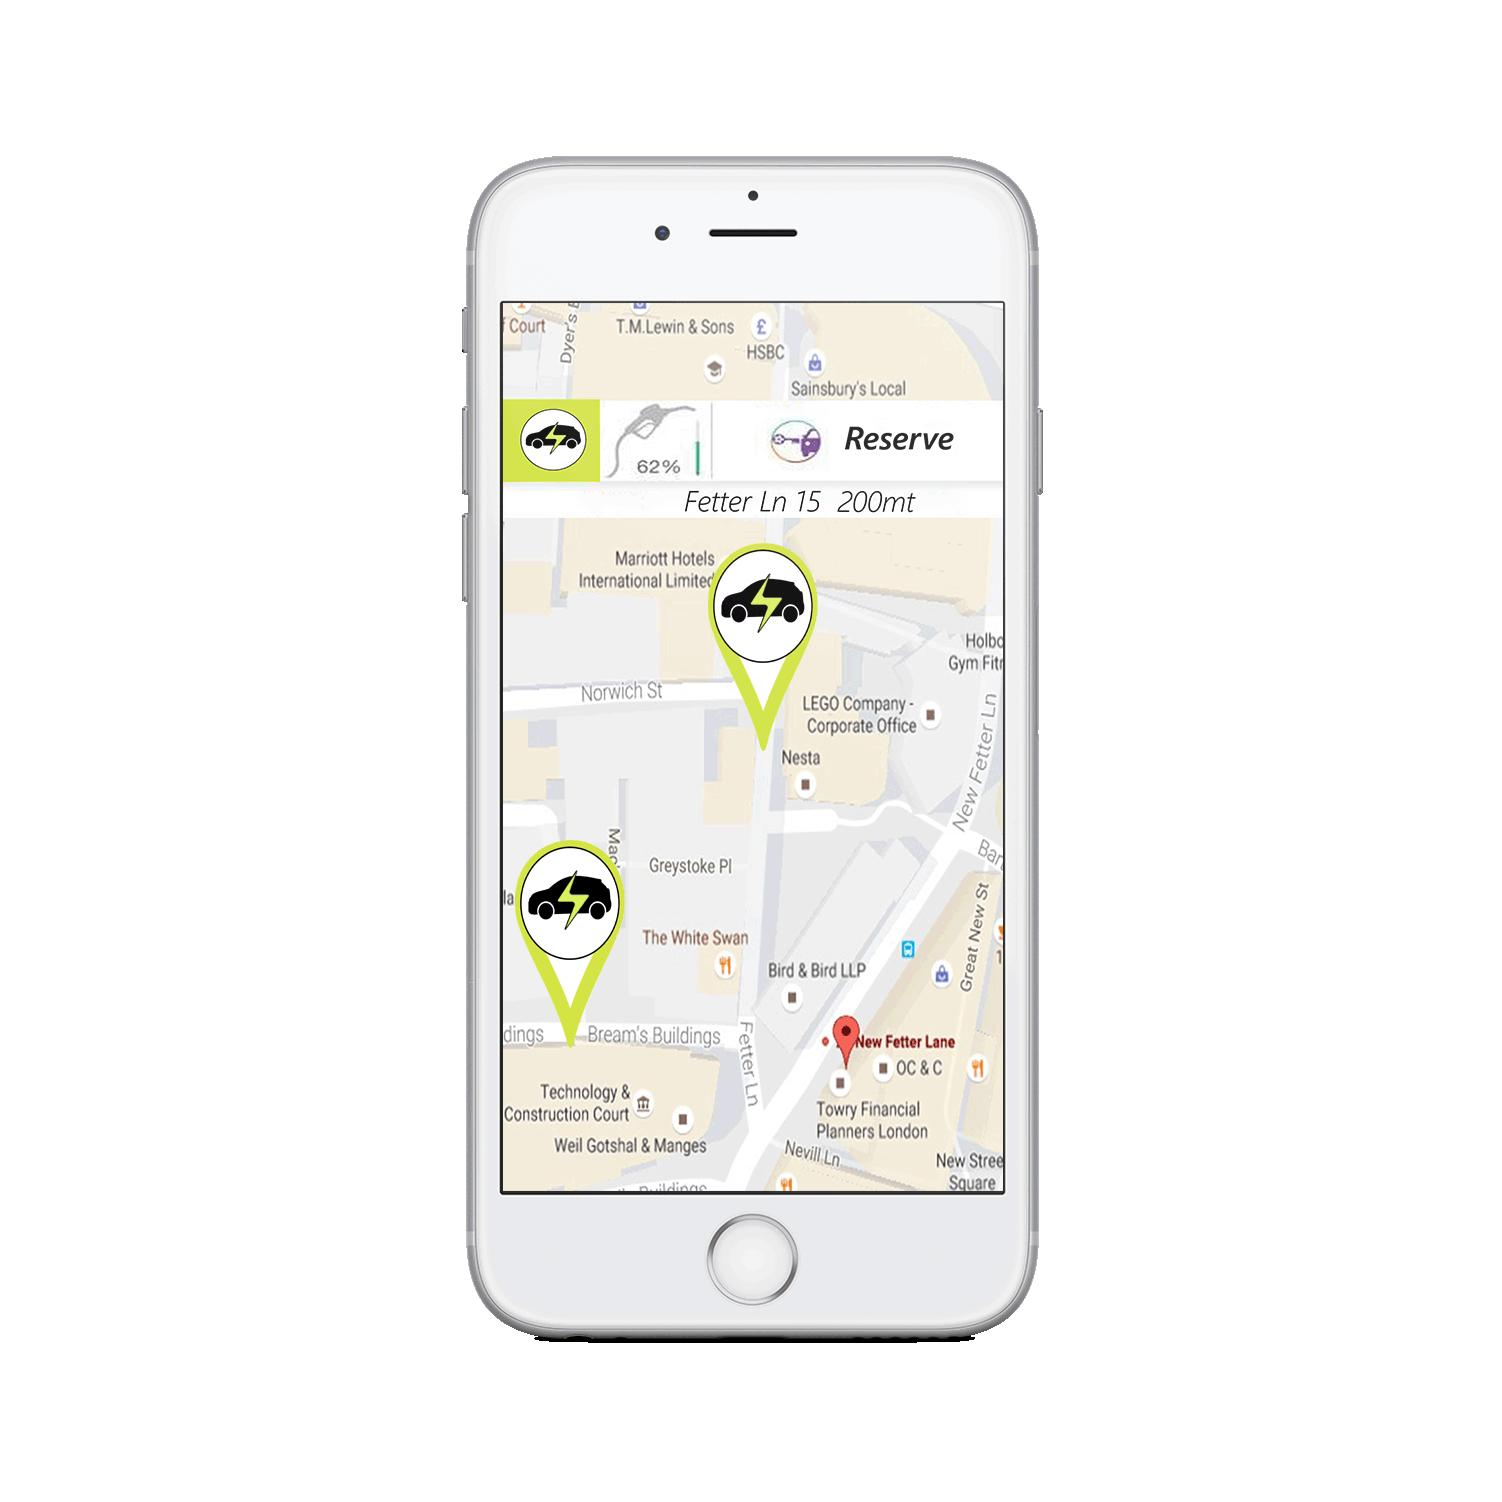
\includegraphics[width=470 pt]{resources/editato.jpg}
\caption{\label{fig:editato}View available car information in mobile application.}
\end{figure}

\newpage

\subsubsection*{View map on the website} This mockup shows the map that a generic user (guest or client) can see on the PowerEnJoy website. On the map are displayed the boundaries of the safe areas in which a client can leave the car and the charging stations with the number of available charging spots. The user can insert an address in order to see the available cars within a certain distance.
\begin{figure}[hp]
\centering
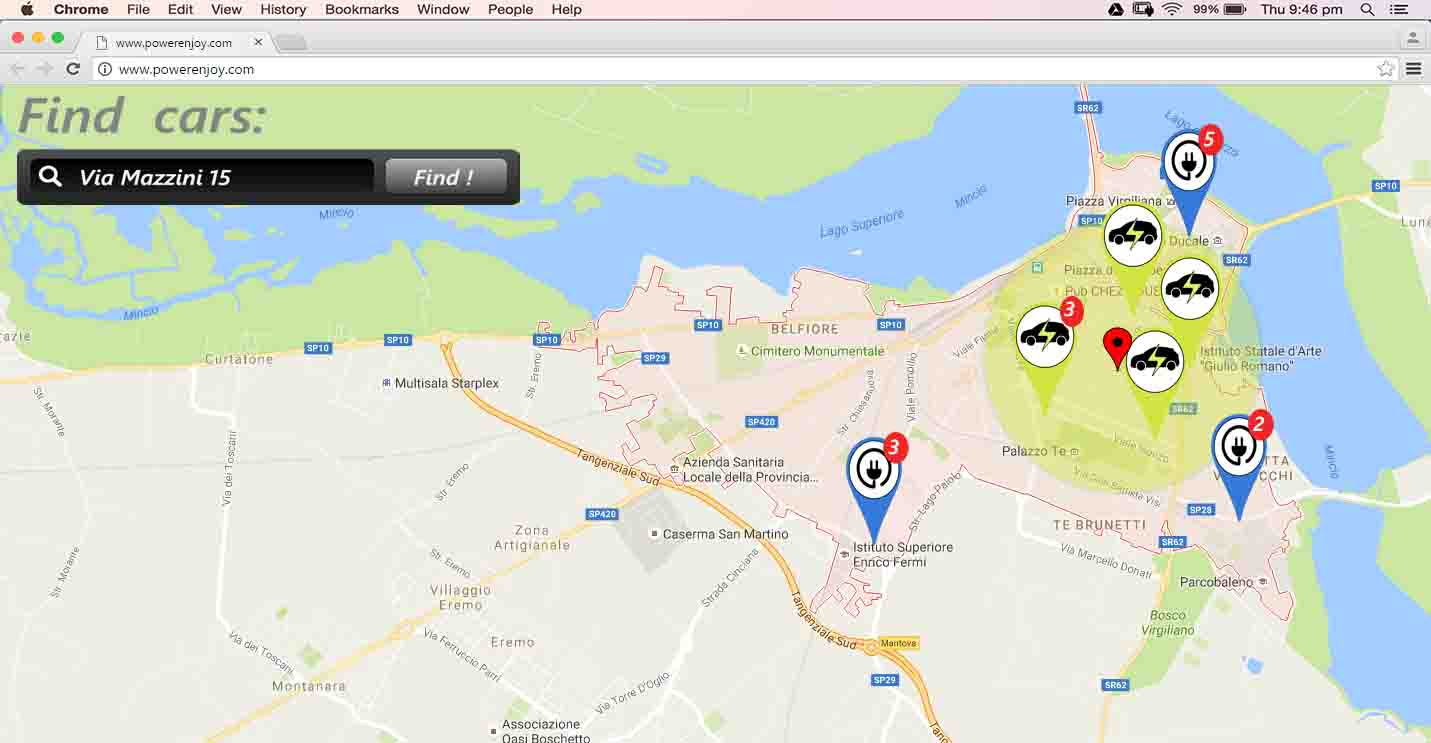
\includegraphics[width=450 pt]{resources/mappa.jpg}
\caption{\label{fig:mappa}View map on the website.}
\end{figure}

\newpage

\subsubsection*{Registration form} The mockup above shows the registration procedure that a guest has to complete in order to become a client and have access to the PowerEnJoy car sharing.

\begin{figure}[hp]
\centering
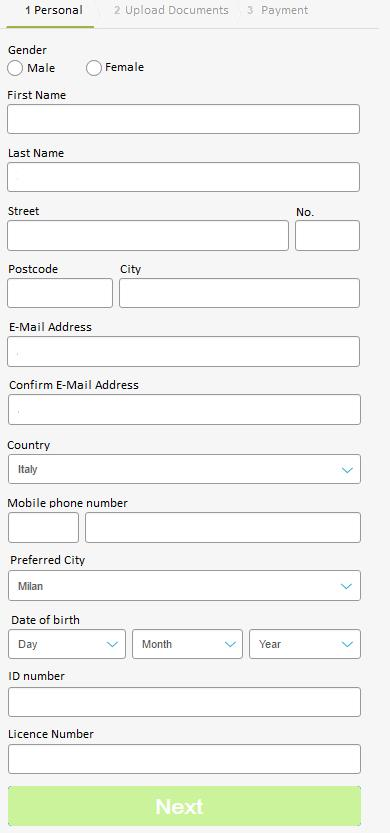
\includegraphics[height=525 pt]{resources/registrazione.jpg}
\caption{\label{fig:reg}Registration form.}
\end{figure}

\newpage

\subsubsection*{Insert pin on the car display} This mockup shows the form in which the client has to insert his pin. After inserting the correct pin the client can start the engine of the car.

\begin{figure}[hp]
\centering
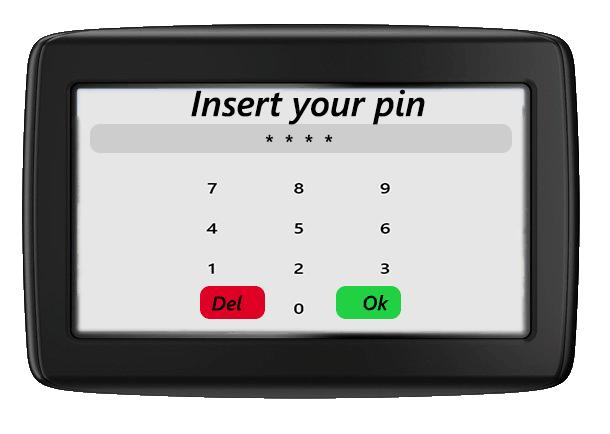
\includegraphics[width=400 pt]{resources/nav68.jpg}
\caption{\label{fig:pin}Insert pin on the car display.}
\end{figure}

\newpage
\subsection{UX Diagrams}
\subsubsection*{UX diagram mobile app}
\begin{figure}[hp]
\centering
\includegraphics[width=400 pt]{resources/UXdiagramApp.jpg}
\caption{\label{fig:uxApp}User Experience diagram app.}
\end{figure}

\newpage
\subsubsection*{UX diagram car}
\begin{figure}[hp]
\centering
\includegraphics[width=400 pt]{resources/UXcar.jpg}
\caption{\label{fig:uxCar}User Experience diagram car.}
\end{figure}

\newpage
\subsection{BCE Diagrams}
\begin{figure}[hp]
\centering
\includegraphics[width=440 pt]{resources/BCE.jpg}
\caption{\label{fig:bce}BCE diagram.}
\end{figure}